\section{Проектирование системы}\label{sec:part2}
Система в целом должна состоять из textbf{клиента}, textbf{сервера} и textbf{БД}.
Общая схема отображена на рисунке \ref{fig:mainArchitecture}.

\begin{figure}[ht]
    \centering
    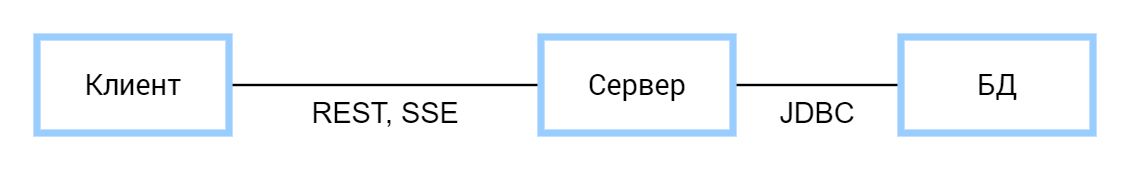
\includegraphics[width=0.9\textwidth]{../resources/mainSystem.png}
    \caption{Общая архитектура приложения.}
    \label{fig:mainArchitecture}
\end{figure}

\subsection{Архитектура БД}
Современные программные системы редко обходятся без энергонезависимого хранилища данных.
Это могут быть реляционные, нереляционные (NoSQL), графовые БД.
В конце концов данные можно хранить в простых текстовых файлах.

В разрабатываемой системе используется реляционная БД.
Это самый простой, хорошо изученный и понятный способ хранить данные.
В контексте этого приложения нет смысла использовать NoSQL решения, основные преимущества которых, а именно высокая гибкость, попросту бессмысленны в данной системе.

\begin{figure}[ht]
    \centering
    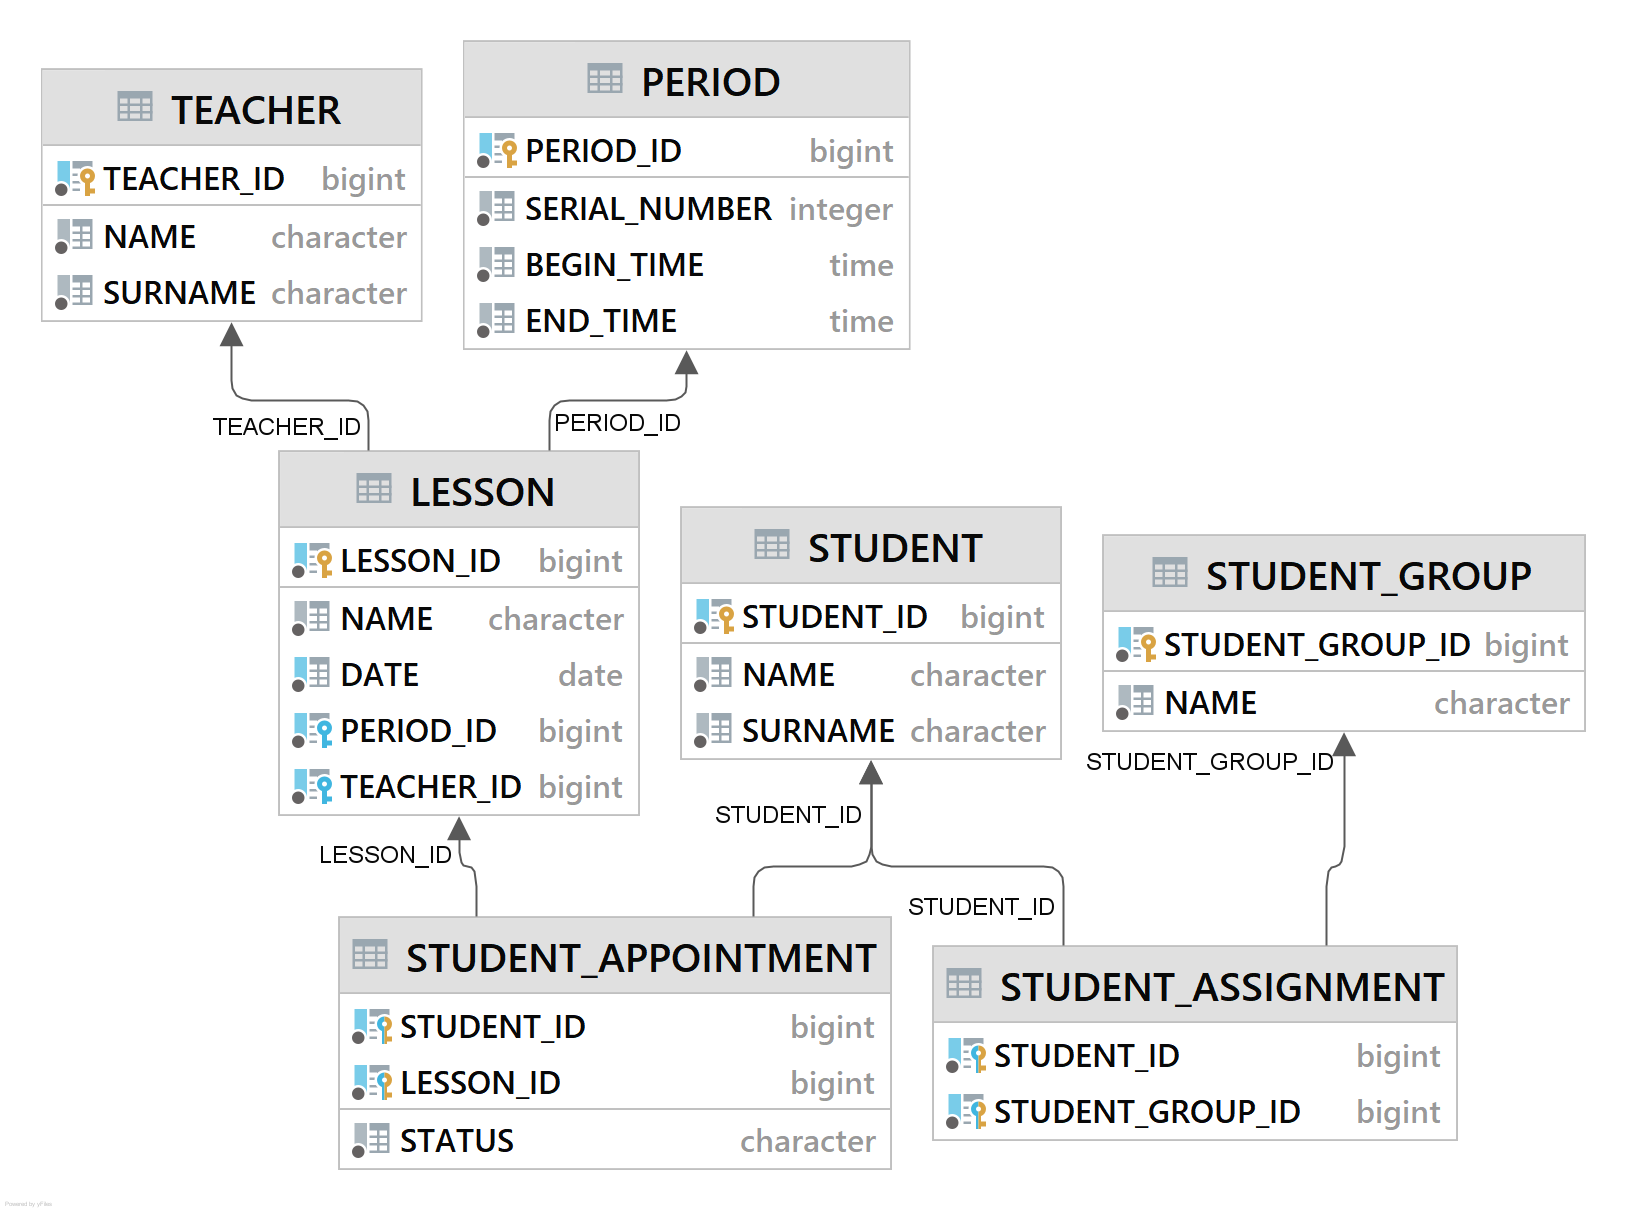
\includegraphics[width=0.9\textwidth]{../resources/schemaSQL.png}
    \caption{Общая архитектура приложения.}
    \label{fig:mainDBArchitecture}
\end{figure}

Как видно на рисунке \ref{fig:mainDBArchitecture}, основные сущности: STUDENT, LESSON, TEACHER, STUDENT\_GROUP.
\begin{itemize}
    \item STUDENT\_GROUP позволяет создавать группы студентов, при этом STUDENT и STUDENT\_GROUP связаны отношением Many-to-many, что позволяет удобно назначать занятие сразу множеству студентов.
    \item STUDENT\_APPOINTMENT хранит статус посещения занятия студентом.
    \item Каждый LESSON связан с PERIOD. PERIOD здесь выступает номером занятия (1-ая, 2-ая пара и т.д.)
\end{itemize}

В качестве конкретной БД использована H2, как простое in-memory решение, что сильно ускоряет разработку.
В боевом применении лучше использовать H2 в Server или Mixed режиме, также хорошим выбором будет PostgreSQL.

\subsection{Архитектура сервера}
Серверная сторона должна отвечать следующим критериям:

\begin{itemize}
    \item Достаточные познания меня, как разработчика, в выбранной платформе.
    \item Возможность легко взаимодействовать с реляционной БД
    \item Удобные инструменты реализации REST API
    \item Поддержка Server Sent Events (SSE)
    \item Доступные инструменты разработки
    \item Простота включения внешних библиотек в приложение
\end{itemize}

К критериям выше идеально подходит Java-Spring \cite{SpringReference} платформа.
Общая схема сервера на Spring выглядит следующим образом:

\begin{figure}[ht]
    \centering
    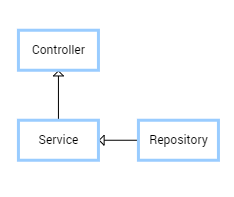
\includegraphics[width=0.6\textwidth]{../resources/serverArchitecture.png}
    \caption{Общая архитектура сервера.}
    \label{fig:mainServerArchitecture}
\end{figure}

\begin{itemize}
    \item Controller формирует REST API, также отвечает за создание SSE.
          При получении HTTP запроса, в этом модуле формируются соответствующие Data Transfer Object (DTO),
          поля DTO валидируются, после управление передается в Service.
    \item Service выполняет в первую очередь связующую функцию.
          Он обращается к Repository и Model по необходимости.
          Также инфраструктурные задачи лежат в основном на Service.
    \item Repository отвечает на взаимодействие с БД.
          В этом слое объекты данные, превращаются в SQL запросы, а результаты этих запросов --- в объекты Model.
    \item В Model хранится бизнес-логика сервера.
\end{itemize}

\subsubsection{Repository}
Для взаимодействия с БД в Java обычно используют JPA, в частности Hibernate \cite{HibernateReference}.
В Spring даже есть абстракция над JPA --- Spring Data JPA \cite{SpringDataJPAReference}.
Но, для реализации поставленной задачи Hibernate, со своей автогенерацией схемы БД, многоуровневым кэшем, дополнительным языком HQL для абстракции над SQL, ленивой подгузкой объектов, также с непонятными SQL-запросами, взявшимися непонятно откуда, кардинально увеличит сложность всего проекта.
К тому же я не очень люблю использовать Hibernate из-за того, что он, по факту, заставляет создавать двунаправленный граф объектов, повторяя схему БД, это приводит к раздуванию сервисов, что плачевно сказывается на читаемости кода.

Поэтому, был выбран Spring Data JDBC \cite{SpringDataJDBCReference}, который к Hibernate и JPA не имеет никакого отношения.
Здесь используется Domain Driven Design (DDD) \cite{EricEvansDDD}, уменьшая размер сервисного слоя, но увеличивая слой доменной модели.
DDD предлагает не строить двунаправленный граф объектов, а использовать паттерн Aggregate Root.
Такой подход позволяет разделить логику на относительно-связанные части --- агрегаты.
В целом понятность системы растёт, а количество ошибок падает.

\subsection{Build tools}
Сборка современного Java приложение уже давно перестал быть тривиальной задачей.
Причина тому --- невероятное количество используемых библиотек.
Для облегчения сборки и запуска Java приложений используются специальные инструменты.
Самые популярные из них: Apache Ant, Apache Maven, Gradle.

\begin{itemize}
    \item Apache Ant был одним из первых инструментов автоматической сборки проектов для Java.
          Ant --- императивный инструмент, что каждое действие должно быть описано в файле конфигурации (в данном случае XML).
          Это придаёт невероятную гибкость во время сборки, но в тоже время, Ant конфигурация может быть невероятно длинной и сложной.
    \item Apache Maven в отличие от Ant --- полностью декларативный инструмент.
          Начать новый проект на Maven очень просто, ведь он сам знает, как и куда загружать зависимости проекта, где находится XML конфигурация самого Maven и т.д.
          От программиста требуется всего-лишь следовать его ожиданиям.
          Слабая сторона Maven --- кастомизация.
          Для задания дополнительной логики необходимо использовать Maven-плагины, которые не всегда полностью покрывают требования.
    \item Gradle находит баланс между императивностью Ant и декларативностью Maven.
          В Gradle отказались от XML заменив его Domain Specific Language (DSL).
          DSL позволяет декларативно описать сборку на Maven, а если нужно, то написать живой код на Groovy или Kotlin (каждый из которых является JVM языком).
\end{itemize}

Для проекта выбран Gradle, как одновременно простой, но гибкий инструмент.
Gradle также предоставляет разбить цельное приложение на модули.

\begin{figure}[ht]
    \centering
    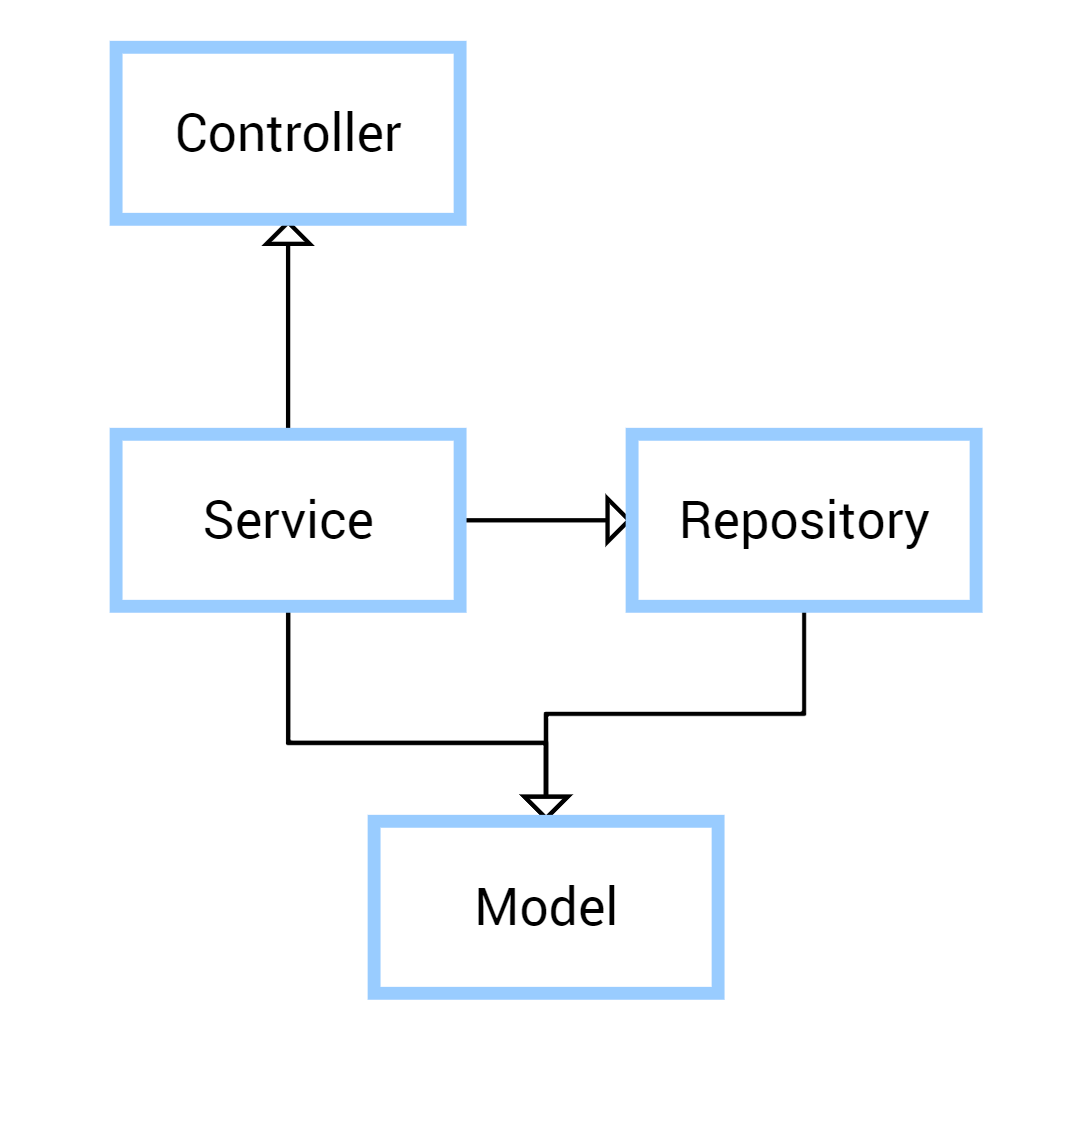
\includegraphics[width=0.6\textwidth]{../resources/moduleDependencies.png}
    \caption{Зависимости модулей друг от друга.}
    \label{fig:moduleDependencies}
\end{figure}

